\documentclass[a4paper]{scrreprt}

% Uncomment to optimize for double-sided printing.
% \KOMAoptions{twoside}

% Set binding correction manually, if known.
% \KOMAoptions{BCOR=2cm}

% Localization options
\usepackage[english]{babel}
\usepackage[T1]{fontenc}
\usepackage[utf8]{inputenc}

% Quotations
\usepackage{dirtytalk}

% Floats
\usepackage{float}

\usepackage{numbertabbing}

% Enhanced verbatim sections. We're mainly interested in
% \verbatiminput though.
\usepackage{verbatim}

% Automatically remove leading whitespace in lstlisting
\usepackage{lstautogobble}

% PDF-compatible landscape mode.
% Makes PDF viewers show the page rotated by 90°.
\usepackage{pdflscape}

% Advanced tables
\usepackage{array}
\usepackage{tabularx}
\usepackage{longtable}

% Fancy tablerules
\usepackage{booktabs}

% Graphics
\usepackage{graphicx}

% Current time
\usepackage[useregional=numeric]{datetime2}

% Float barriers.
% Automatically add a FloatBarrier to each \section
\usepackage[section]{placeins}

% Custom header and footer
\usepackage{fancyhdr}

\usepackage{geometry}
\usepackage{layout}

% Math tools
\usepackage{mathtools}
% Math symbols
\usepackage{amsmath,amsfonts,amssymb}
\usepackage{amsthm}

\DeclarePairedDelimiter\ceil{\lceil}{\rceil}
\DeclarePairedDelimiter\floor{\lfloor}{\rfloor}

% General symbols
\usepackage{stmaryrd}

\DeclarePairedDelimiter\abs{\lvert}{\rvert}

% Indistinguishable operator (three stacked tildes)
\newcommand*{\diffeo}{% 
  \mathrel{\vcenter{\offinterlineskip
  \hbox{$\sim$}\vskip-.35ex\hbox{$\sim$}\vskip-.35ex\hbox{$\sim$}}}}

% Bullet point
\newcommand{\tabitem}{~~\llap{\textbullet}~~}

\floatstyle{ruled}
\newfloat{algo}{htbp}{algo}
\floatname{algo}{Algorithm}
% For use in algorithms
\newcommand{\str}[1]{\textsc{#1}}
\newcommand{\var}[1]{\textit{#1}}
\newcommand{\op}[1]{\textsl{#1}}

\pagestyle{plain}
% \fancyhf{}
% \lhead{}
% \lfoot{}
% \rfoot{}
% 
% Source code & highlighting
\usepackage{listings}

% SI units
\usepackage[binary-units=true]{siunitx}
\DeclareSIUnit\cycles{cycles}

% Convenience commands
\newcommand{\mailsubject}{33107 - Document Image Analysis - Series 2}
\newcommand{\maillink}[1]{\href{mailto:#1?subject=\mailsubject}
                               {#1}}

% Should use this command wherever the print date is mentioned.
\newcommand{\printdate}{\today}

\subject{33107 - Document Image Analysis}
\title{Series 2}

\author{Michael Senn \maillink{michael.senn@students.unibe.ch} - 16-126-880}

\date{\printdate}

% Needs to be the last command in the preamble, for one reason or
% another. 
\usepackage{hyperref}

\begin{document}
\maketitle


\setcounter{chapter}{1}

\chapter{Series 2}

\section{Notation}

Unless noted otherwise, assume the following definitions for arithmetic operations:
\begin{itemize}
		\item On two scalars: The usual definition in $\mathbb{R}$
		\item On two matrices of equal shape: Pairwise operation in $\mathbb{R}$.
				Result is a matrix of shape equal to the inputs.
		\item On a scalar and a matrix: Pairwise operation on each element of the
				matrix with the scalar in $\mathbb{R}$. Result is a matrix of
				shape equal to the input one.
\end{itemize}

\section{GitHub repository}

The code can be found at \url{https://github.com/Lavode/33107-document-image-analysis}

\section{Features for MNIST classification}

The following features were chosen to be evaluated for classifying handwritten
digits from the MNIST sample set. For all algorithms consider a $28 \times 28$
image $I$, with $I[y, x], 0 \leq x, y \leq 27$ being the pixel at position $(y,
x)$. Let $x$ be the horizontal, $y$ the vertical coordinate.

Each feature defines two operations - feature extraction, where the feature is
extracted from an input image - and feature comparison, where the extracted
feature of a to-be-classified image is compared with the feature of a class
representative.

\subsection{Average pixel value}

The average pixel value is defined in algorithm \ref{alg:average_pixel}. As a
feature it is unlikely to produce good values, as it is comparable to simply
measuring the area each digit takes up. Since there is a lot of overlap when it
comes to area, it is unlikely to be suitable to differentiate between digits.
None the less it is trivial enough to implement that one might as well.

\begin{algo}
  \vbox{
    \small
    \begin{numbertabbing}
      xxxx\=xxxx\=xxxx\=xxxx\=xxxx\=xxxx\=MMMMMMMMMMMMMMMMMMM\=\kill
	  \textbf{Feature extraction} \\
	  \> \textbf{Input} \\
	  \> \> \var{I}: Input image \\
	  \> \\
	  \> \var{sum} := 0 \\
	  \> \textbf{For} x := 0 to 27 \\
	  \> \> \textbf{For} y := 0 to 27 \\
	  \> \> \> \var{sum} += I[y, x] \\
	  \> \textbf{Return} \var{sum} / (28 * 28) \\
	  \> \\
	  \textbf{Comparison} \\
	  \> \textbf{Input} \\
	  \> \> \var{a}: Average pixel value of representative \\
	  \> \> \var{b}: Average pixel value of image to be classified \\
	  \> \\
	  \> \textbf{Return} |a - b| / 256
    \end{numbertabbing}
  }
  \caption{Average pixel value} 
  \label{alg:average_pixel}
\end{algo}

\subsection{Horizontal profile}

The horizontal profile is described in algorithm \ref{alg:horizontal_profile}.
It is expected to provide good results for digits with a distinct horizontal
profile such as a 1, and less good results for digits with more complex and
less distinct profiles such as a 5 or 6.

\begin{algo}
  \vbox{
    \small
    \begin{numbertabbing}
      xxxx\=xxxx\=xxxx\=xxxx\=xxxx\=xxxx\=MMMMMMMMMMMMMMMMMMM\=\kill
	  \textbf{Feature extraction} \\
	  \> \textbf{Input} \\
	  \> \> \var{I}: Input image \\
	  \> \\
	  \> \var{profile} := Matrix of shape (28, 1) \\
	  \> \textbf{For} x := 0 to 27 \\
	  \> \> \textbf{For} y := 0 to 27 \\
	  \> \> \> \var{profile}[x] += I[y, x] \\
	  \> \textbf{Return} \var{profile} / 28 \\
	  \> \\
	  \textbf{Comparison} \\
	  \> \textbf{Input} \\
	  \> \> \var{a}: Horizontal profile of representative \\
	  \> \> \var{b}: Horizontal profile of image to be classified \\
	  \> \\
	  \> \textbf{Return} |a - b| / 256
    \end{numbertabbing}
  }
  \caption{Horizontal profile} 
  \label{alg:horizontal_profile}
\end{algo}


\subsection{Vertical profile}

The vertical profile is described in algorithm \ref{alg:vertical_profile}.  It
is expected to provide good results for digits with a distinct vertical profile
such as a 1 or 8, and less good results for digits with more complex and less
distinct profiles such as a 2 or 5.

\begin{algo}
  \vbox{
    \small
    \begin{numbertabbing}
      xxxx\=xxxx\=xxxx\=xxxx\=xxxx\=xxxx\=MMMMMMMMMMMMMMMMMMM\=\kill
	  \textbf{Feature extraction} \\
	  \> \textbf{Input} \\
	  \> \> \var{I}: Input image \\
	  \> \\
	  \> \var{profile} := Matrix of shape (28, 1) \\
	  \> \textbf{For} y := 0 to 27 \\
	  \> \> \textbf{For} x := 0 to 27 \\
	  \> \> \> \var{profile}[y] += I[y, x] \\
	  \> \textbf{Return} \var{profile} / 28 \\
	  \> \\
	  \textbf{Comparison} \\
	  \> \textbf{Input} \\
	  \> \> \var{a}: Vertical profile of representative \\
	  \> \> \var{b}: Vertical profile of image to be classified \\
	  \> \\
	  \> \textbf{Return} |a - b| / 256
    \end{numbertabbing}
  }
  \caption{Vertical profile} 
  \label{alg:vertical_profile}
\end{algo}

\subsection{Euclidean distance}

The euclidean distance described in algorithm \ref{alg:euclidean_distance}
treats the $28 \times 28$ input image as a $28 \cdot 28 = 784$-dimensional
vector, of which the euclidean distance is calculated:

\[
		d(a, b) = \sqrt{(a_1 - b_1)^2 + \ldots + (a_n - b_n)^2}
\]

\begin{algo}
  \vbox{
    \small
    \begin{numbertabbing}
      xxxx\=xxxx\=xxxx\=xxxx\=xxxx\=xxxx\=MMMMMMMMMMMMMMMMMMM\=\kill
	  \textbf{Feature extraction} \\
	  \> \textbf{Input} \\
	  \> \> \var{I}: Input image \\
	  \> \\
	  \> \textbf{Return} \op{Flatten}(I) \\
	  \> \\
	  \textbf{Comparison} \\
	  \> \textbf{Input} \\
	  \> \> \var{a}: $28^2$-dimensional vector of representative \\
	  \> \> \var{b}: $28^2$-dimensional vector of image to be classified \\
	  \> \\
	  \> \var{sum} := 0 \\
	  \> \textbf{For} i := 0 to 783 \\
	  \> \> \var{sum} += $((a[i] - b[i]) / 256)^2$ \\
	  \> \textbf{Return} $\sqrt{sum} / 784$
    \end{numbertabbing}
  }
  \caption{Euclidean distance}
  \label{alg:euclidean_distance}
\end{algo}

\section{Custom classifier}

\begin{itemize}
		\item In a first step, the classifier is trained on the training set
				with the set of chosen features. The features are extracted
				from each sample, and a class representative is calculated as
				the average feature vector over all samples.

		\item In the testing step, the class representatives are then used to
				gauge the `distance' of each to-be-classified image from the
				class representative. With $n$ features and 10 classes this
				leads to a matrix $(d_{ij})$ of shape $(10, n)$, where $d_{ij}$
				is the `distance' of the classified image - in terms of feature
				$j$ - from class $i$.

		\item These are then combined into one distance per class by either the
				mean, or the minimum, operation.

		\item Lastly the class with the lowest distance is chosen
\end{itemize}

The distance values of each feature are normalized to $[0, 1]$ based on their
theoretical range of values. This prevents one feature with a bigger range from
dominating, but does not necessarily lead to ideal results if the value
distribution of one feature is more narrow than another.

A more elaborate approach would be to have each feature report a `certainity'
value per class, of how certain it is that the to-be-classified image belongs
to this class.

\section{Results with custom classifier}

\subsection{Single features}

In a first step, each feature was evaluated on its own. Results are shown in
figure \ref{fig:evaluation_single}. As expected the average-pixel feature
performed awfully except for the digit `1', which has a substantially lower
area than the other digits. For this reason this feature was dropped
immediately.

The horizontal and vertical profiles performed well at identifying digits with
a distinct profile, with the vertical profile usually outperforming, other
times being on par with, the horizontal profile.

The euclidean distance finally outperformed all the other features for every
single digit.

\begin{figure}[h]
        \centering
		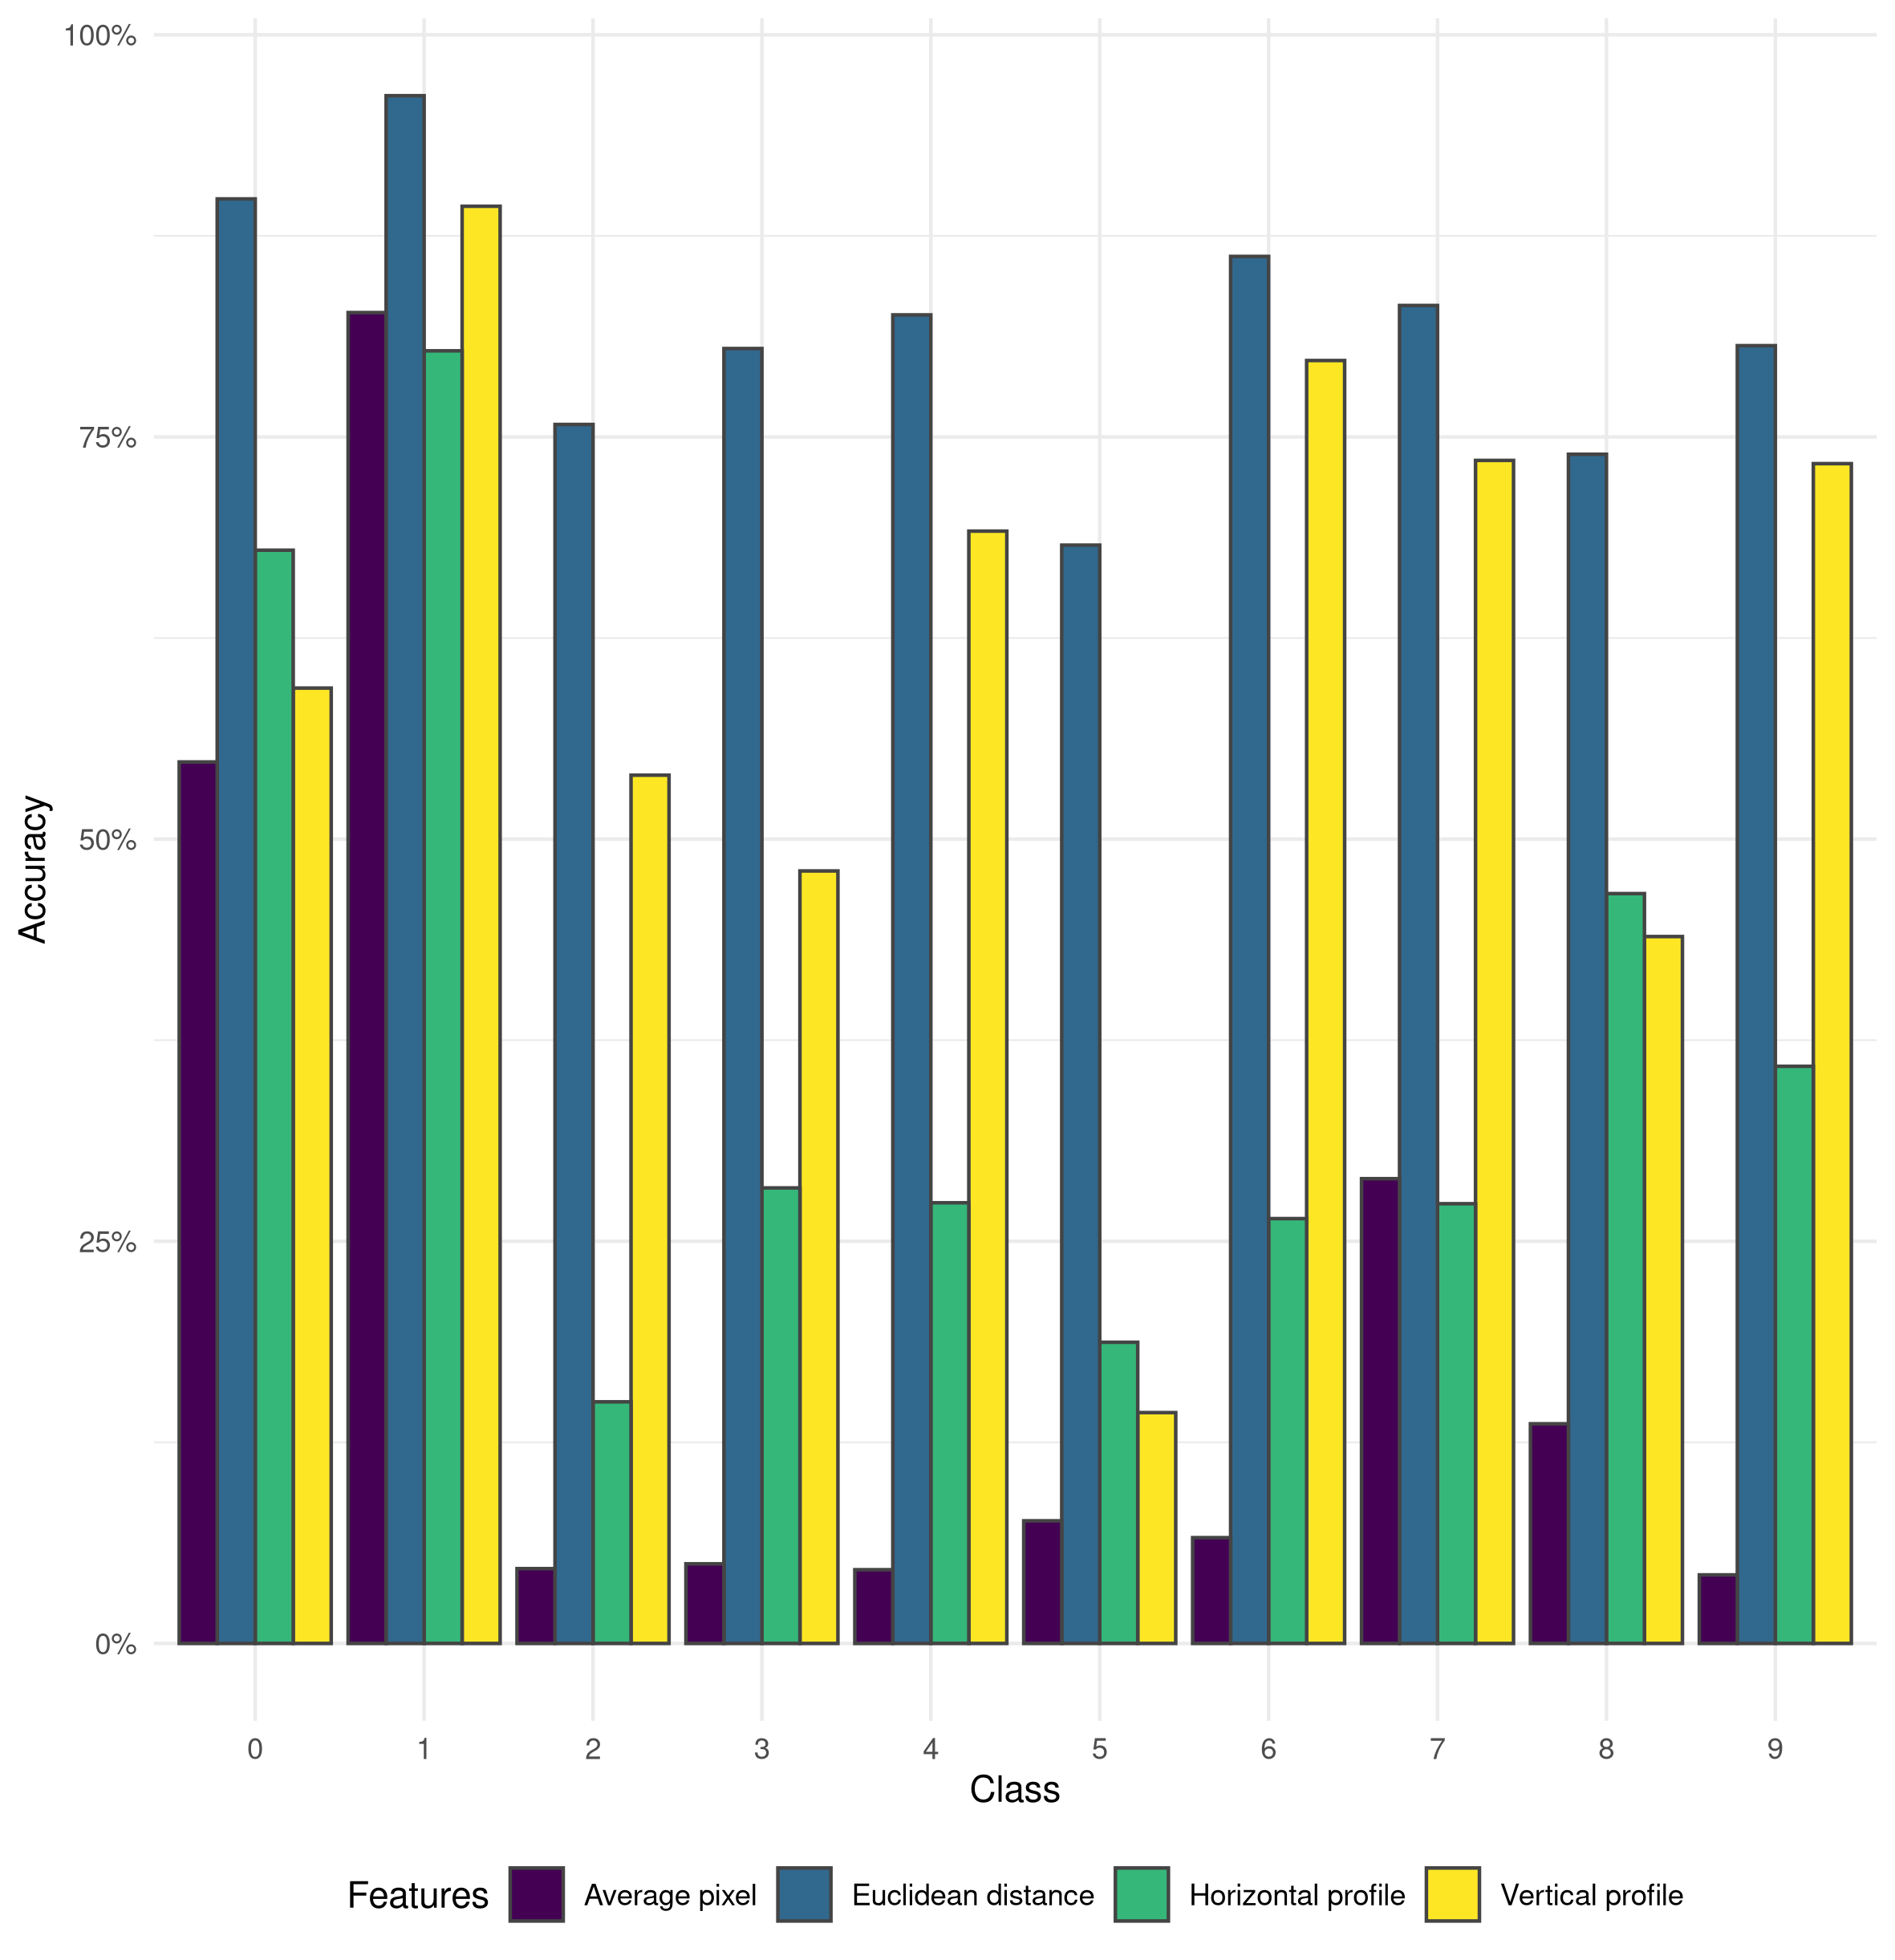
\includegraphics[width=0.8\textwidth]{../resources/features_single.png}
		\caption{Evaluation of single features}
		\label{fig:evaluation_single}
\end{figure}

\subsection{Combining horizontal and vertical profile}

In a second step, the horizontal and vertical profiles were combined and
compared with their standalone usage. Two combinations were tried, one where
the average distance value of the two features was used, and one where the
lower of the two was used. Results are shown in figure
\ref{fig:evaluation_profiles}.

The average of the two performed slightly better than the vertical profile on
some classes, while being on par for others. The minimum of the two performed
consistently worse.

\begin{figure}[h]
        \centering
		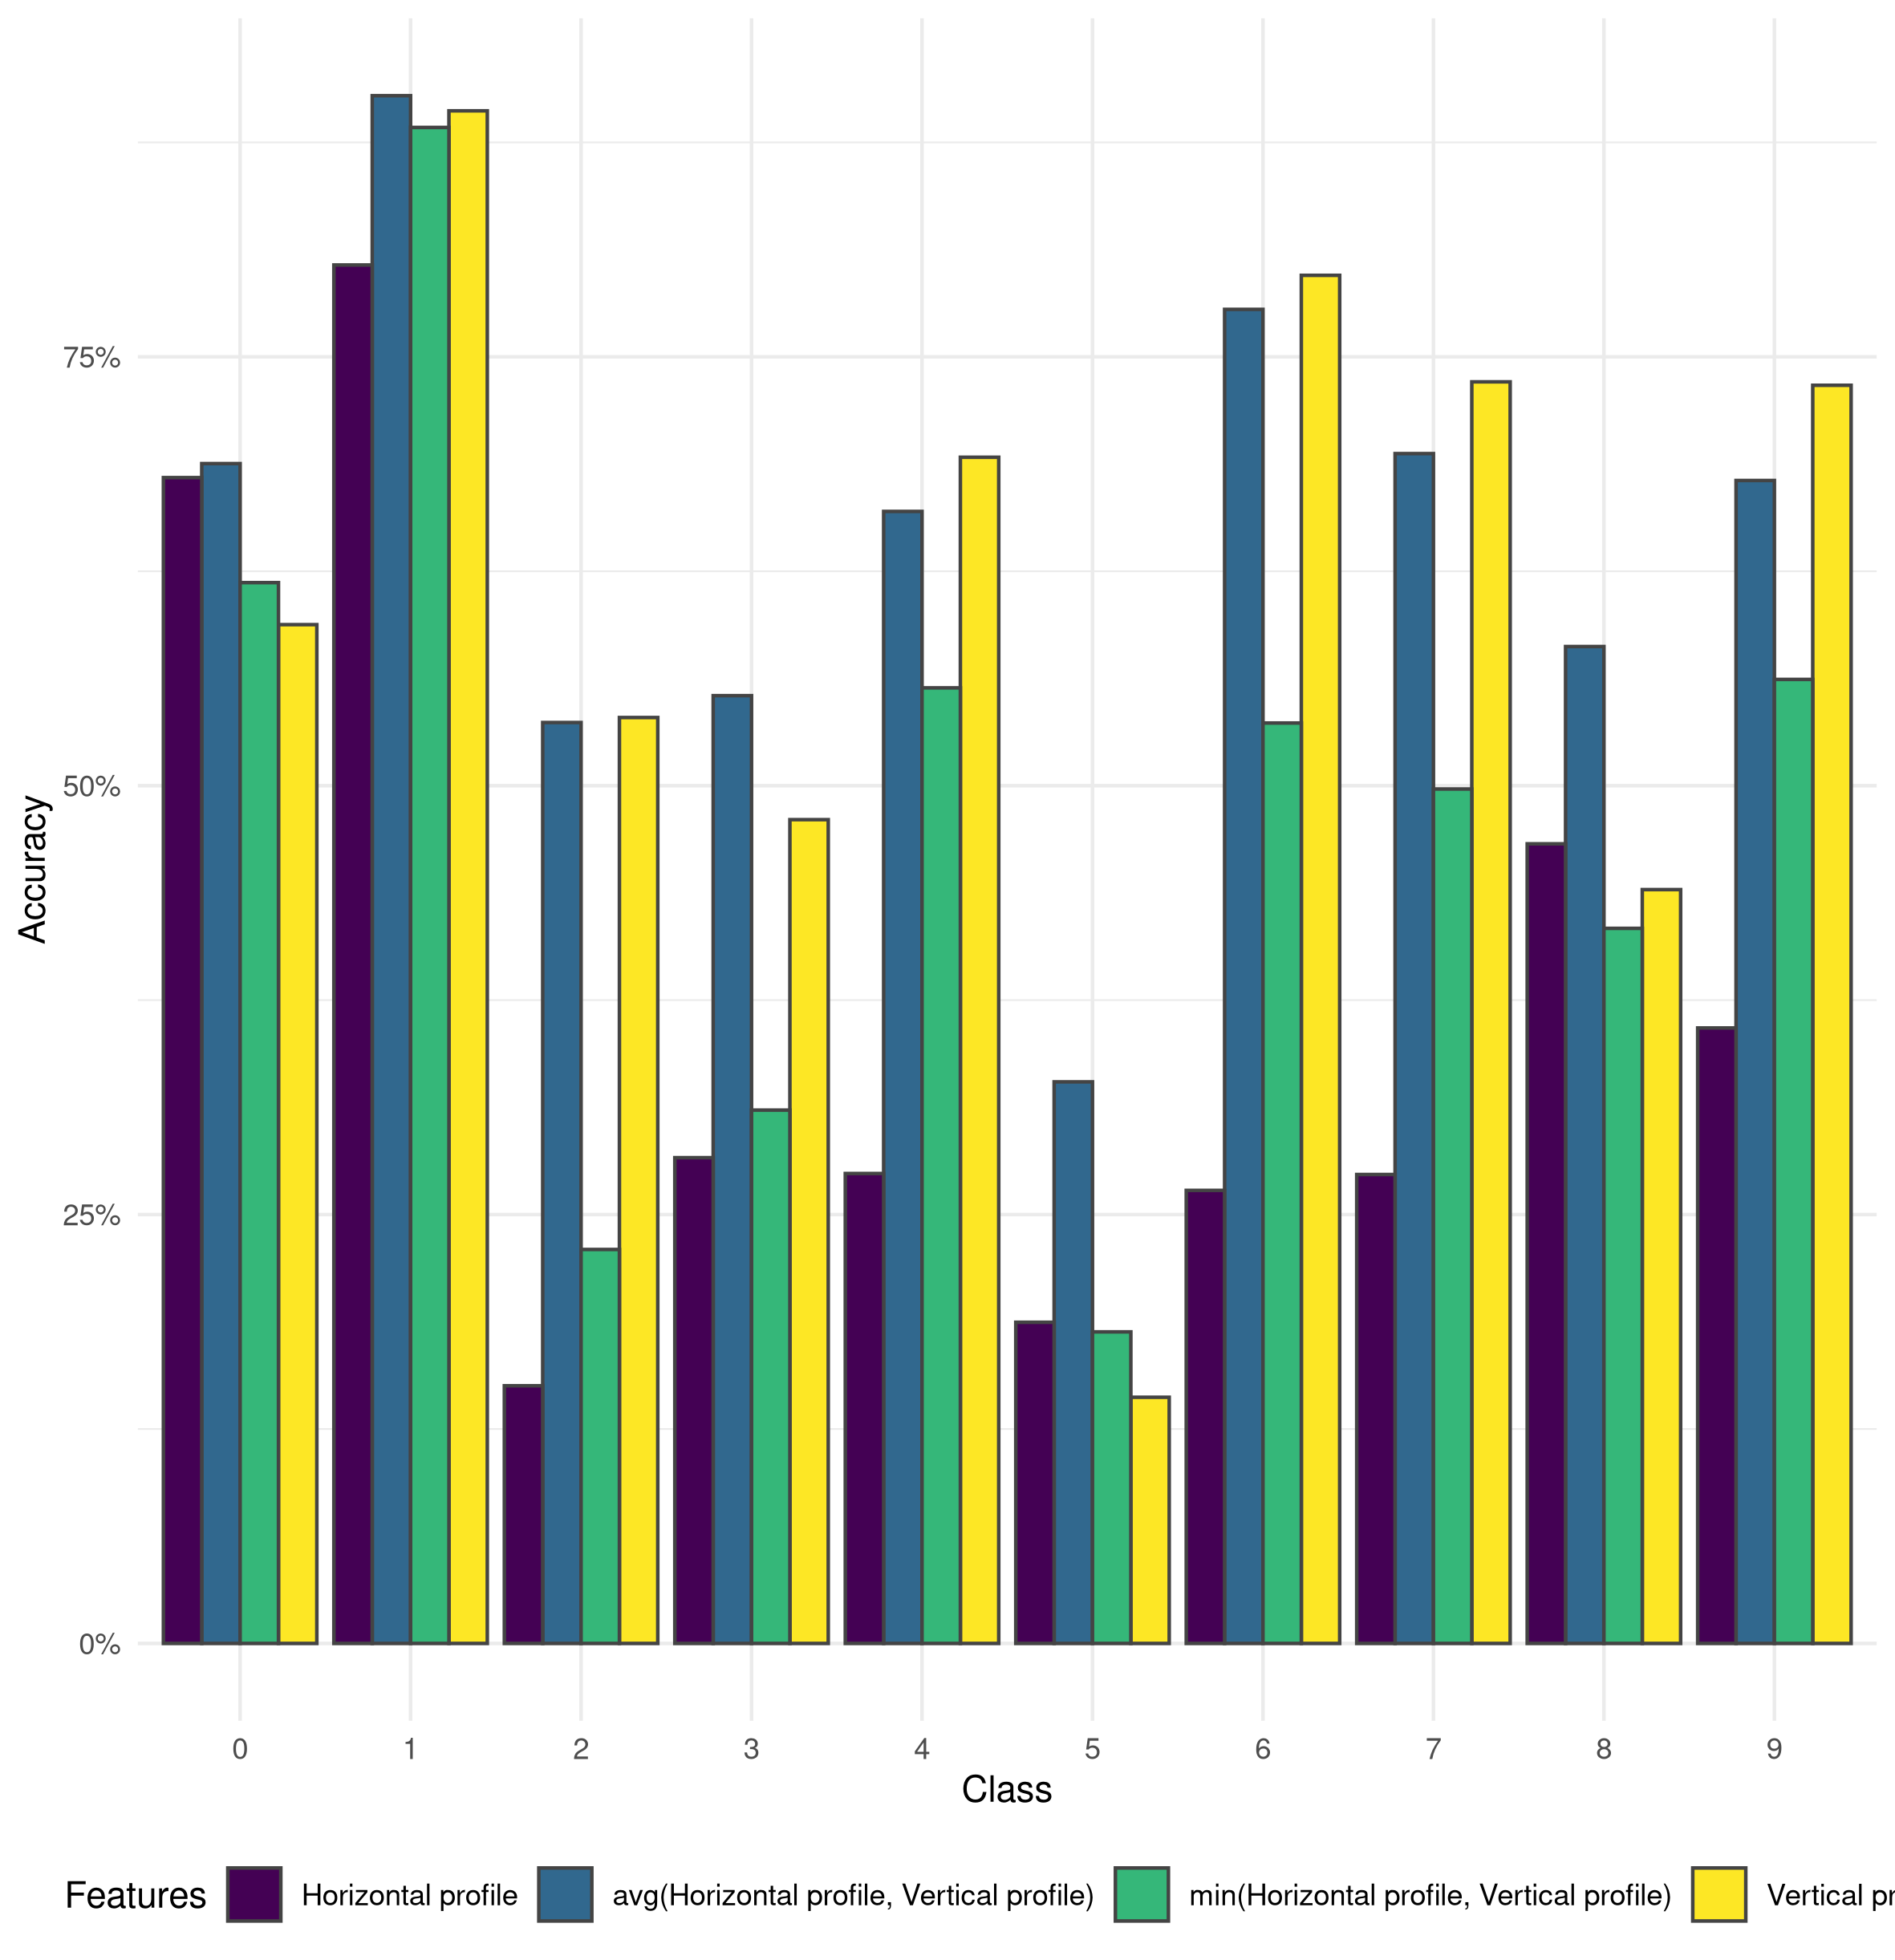
\includegraphics[width=0.8\textwidth]{../resources/features_profiles.png}
		\caption{Evaluation of horizontal \& vertical profile combinations}
		\label{fig:evaluation_profiles}
\end{figure}

\subsection{Top contenders}

Finally, three promising feature sets were compared:
\begin{itemize}
		\item The euclidean distance
		\item The average of horizontal and vertical profile
		\item The average of euclidean distance, horizontal and vertical profile
\end{itemize}

Results are shown in figure \ref{fig:evaluation_top}. The average of the
profiles was outperformed across the board, with the average of the three being
nearly as good as - but always a bit worse than - the euclidean distance alone.

\begin{figure}[h]
        \centering
		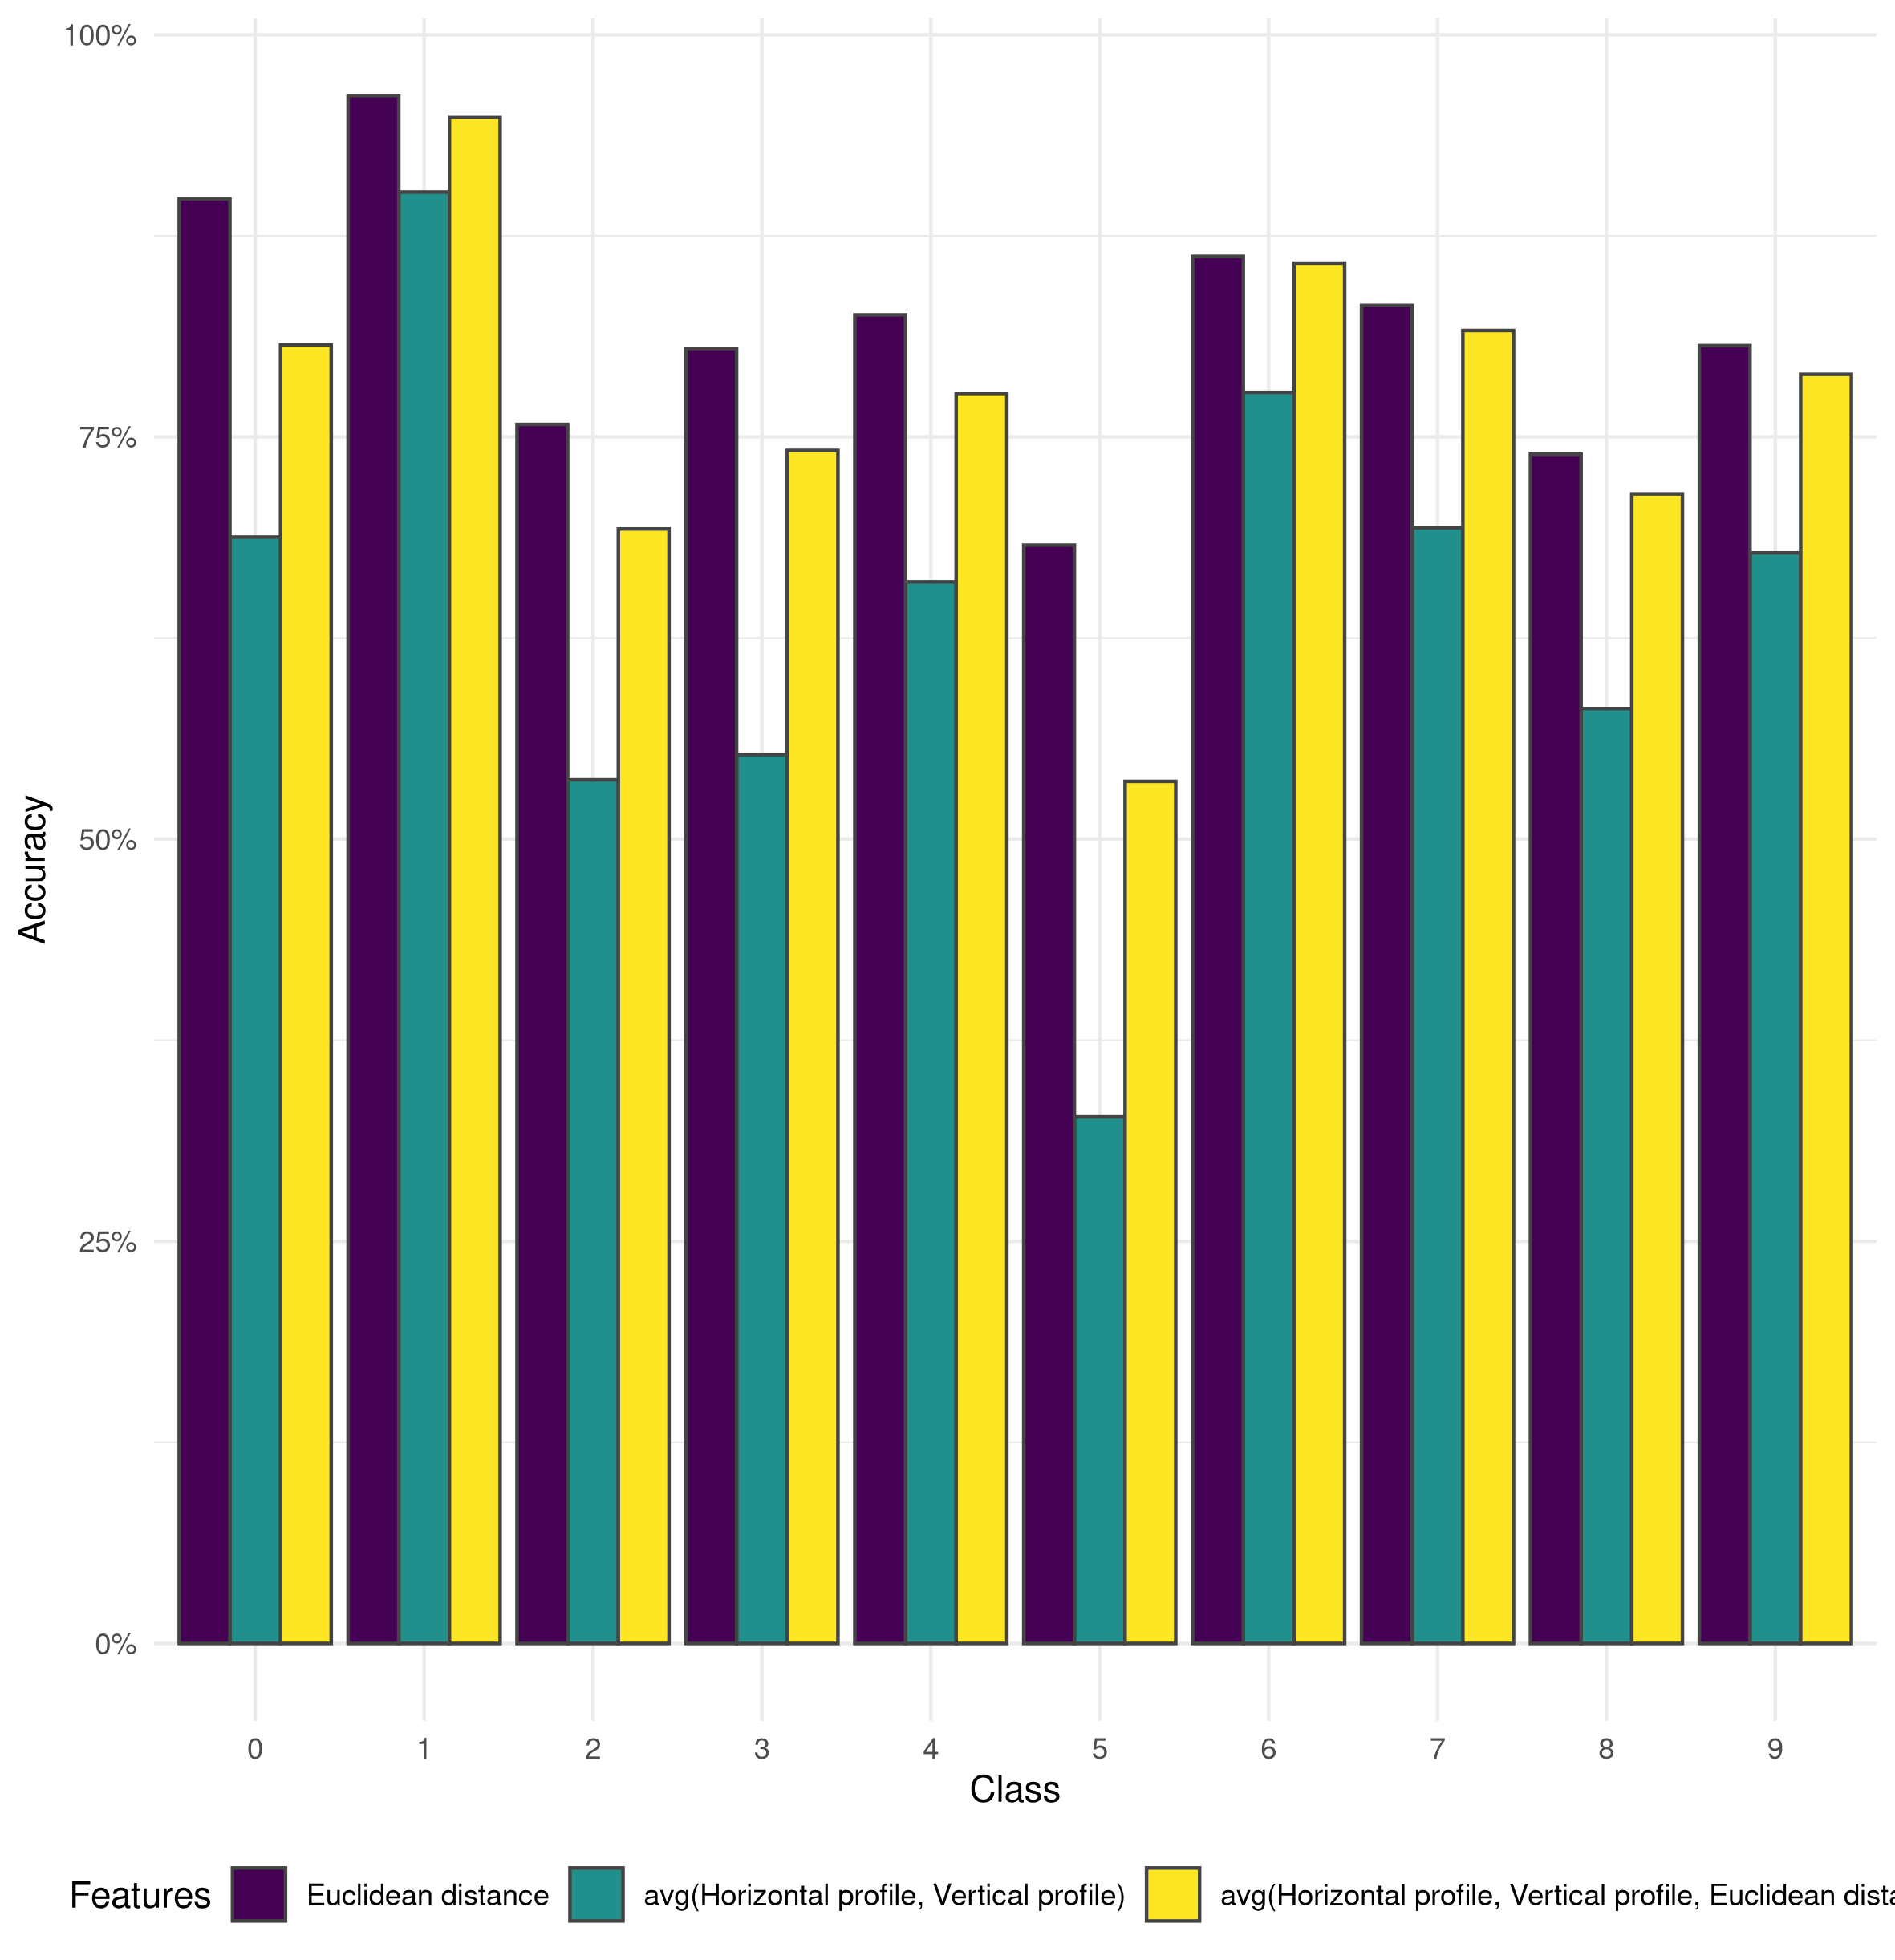
\includegraphics[width=0.8\textwidth]{../resources/features_top.png}
		\caption{Evaluation of top combinations}
		\label{fig:evaluation_top}
\end{figure}

\subsection{Conclusion}

Table \ref{tbl:evaluation} provides some additional statistics on the
accuracies of the feature combinations. As discussed earlier, the euclidean
distance alone lead to the best results. It is possible that a more elaborate
combination of features would lead to results exceeding the single euclidean
distance.

\begin{table}
		\begin{tabular}{lllll}
				\toprule
				Aggregation & Features & Average & Worst & Best \\
				\midrule
				- & Average pixel & \SI{21}{\percent} & \SI{4}{\percent} & \SI{83}{\percent} \\
				- & Horizontal profile & \SI{37}{\percent} & \SI{15}{\percent} & \SI{80}{\percent} \\
				- & Vertical profile & \SI{60}{\percent} & \SI{14}{\percent} & \SI{89}{\percent} \\
				- & Euclidean distance & \SI{82}{\percent} & \SI{68}{\percent} & \SI{96}{\percent} \\
				Avg & H. profile, V. profile & \SI{64}{\percent} & \SI{33}{\percent} & \SI{90}{\percent} \\
				Min & H. profile, V. profile & \SI{48}{\percent} & \SI{18}{\percent} & \SI{88}{\percent} \\
				Avg & H. profile, V. profile, Euclidean distance & \SI{77}{\percent} & \SI{54}{\percent} & \SI{95}{\percent} \\
				\bottomrule
		\end{tabular}
		\label{tbl:evaluation}
		\caption{Feature statistics}
\end{table}

\section{Results with scikit-learn classifiers}

In a last step, some feature sets were tested in combination with standard
classifiers offered by the scikit-learn library. The following classifiers were
evaluated:

\begin{itemize}
		\item K-Neighbors classifier
		\item Linear SVC
		\item Multi-layer perceptron classifier
\end{itemize}

In combination with the following feature sets:

\begin{itemize}
		\item Horizontal \& vertical profile
		\item Raw pixel values as $784$-dimensional vector
		\item Raw pixel values, horizontal \& vertical profile
\end{itemize}

Only feature sets which had performed well with the custom classifier were
considered, to not bloat this any more.

The combination of all three features was not tested with the linear
support-vector classifier, due to training times exceeding half an hour.

\subsection{Standardization}

Both training as well as test data was standardized, that is transformed such
that its mean was $0$ and its variance $1$. This is required for proper
training with some models such as support-vector classifiers, and does not hurt
accuracy with other classifiers.

\subsection{Runtime}

\subsubsection{Feature extraction}

Runtime for feature extraction is independent from the choice of classifier,
and as such was the same for all. Feature extraction took an average of
\SI{3.5}{\s}, though this also involved disk access which is likely to have
dominated the metric.

\subsubsection{Training the classifier}

The runtime to train the various classifiers on the full training set of 48000
samples is shown in figure \ref{fig:training_time}.

Training the K-Neighbors classifier took only fractions of a second which is to
be expected, as its training phase merely consists of storing the training
data. Training time of the linear SVC was highly dependant on the number of
features, with training on the full pixel data taking roughly half an hour.
Training the MLP was largely independant of the number of features, taking
around \SI{100}{\s} consistently.

\begin{figure}[h]
        \centering
		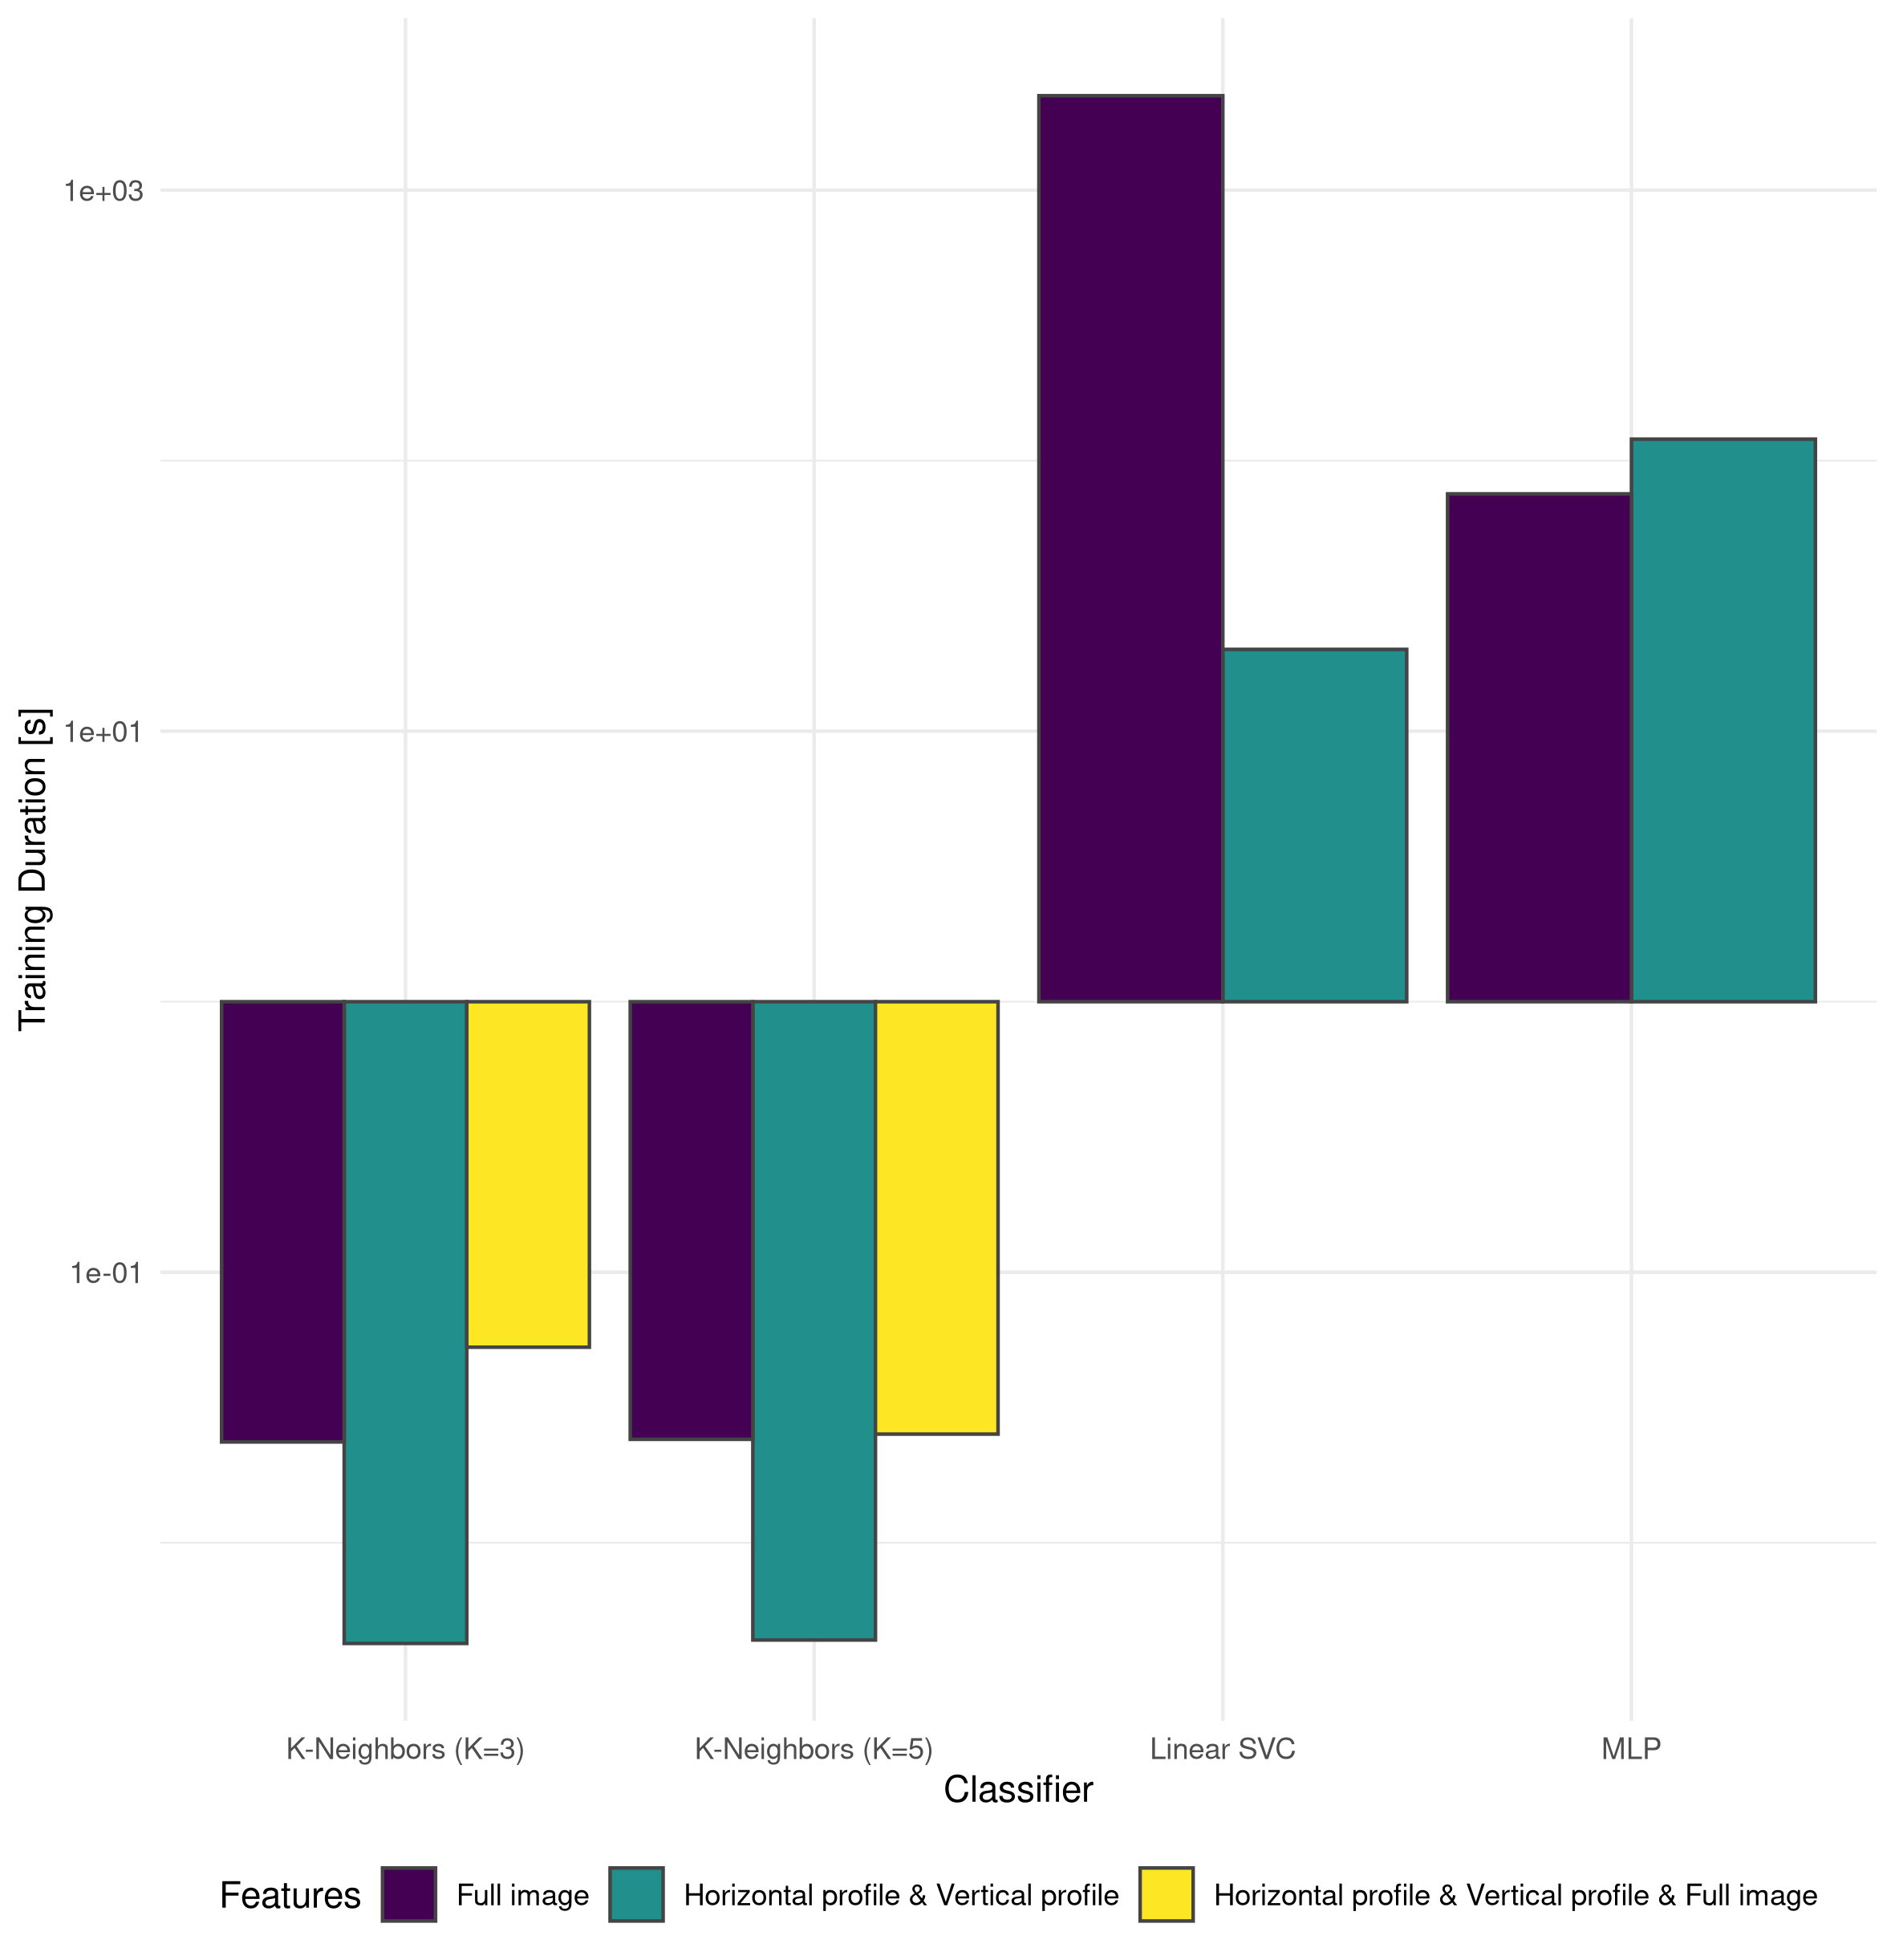
\includegraphics[width=0.8\textwidth]{../resources/scikit_training_timings.png}
		\caption{Training time}
		\label{fig:training_time}
\end{figure}

\subsubsection{Prediction}

Figure \ref{fig:prediction_time} shows the average prediction time per test
sample. The K-neighbors classifier took around \SI{1e-3}{\s} per sample, with
the linear SVC and MLP classifiers being about three to four orders of
magnitude faster.

\begin{figure}[h]
        \centering
		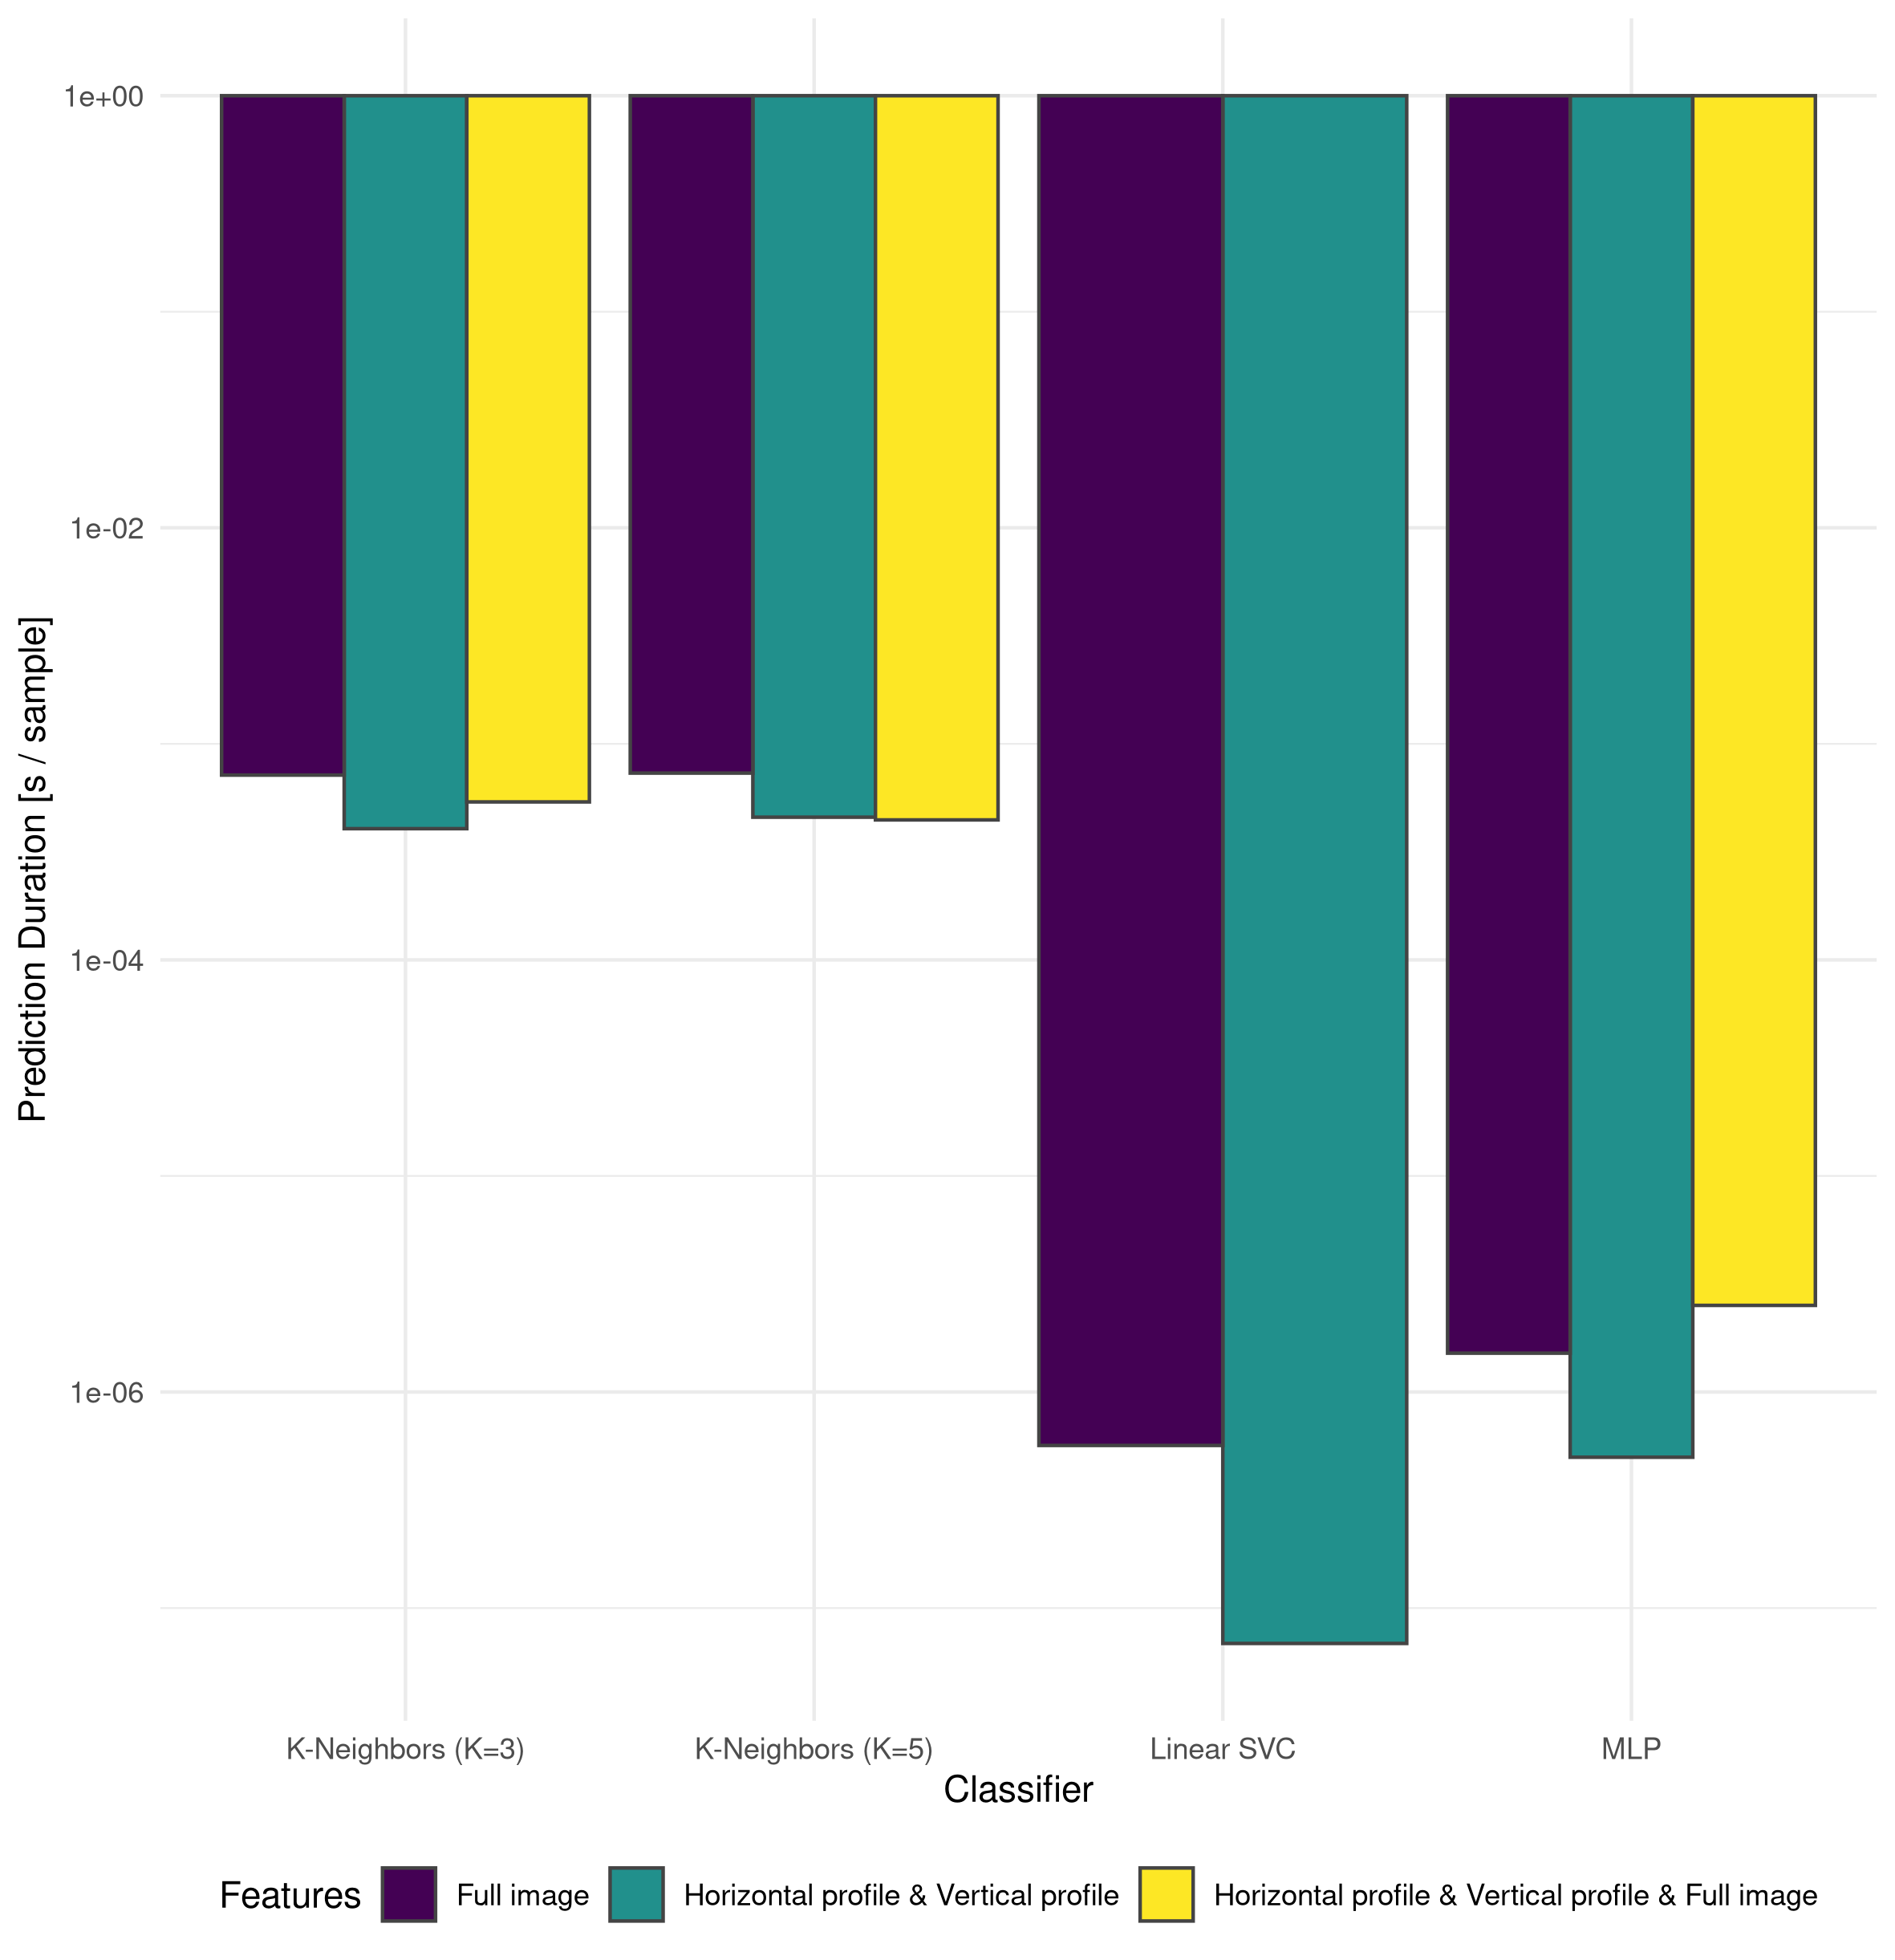
\includegraphics[width=0.8\textwidth]{../resources/scikit_prediction_timings.png}
		\caption{Prediction time}
		\label{fig:prediction_time}
\end{figure}

\subsection{Prediction accuracy}

Figure \ref{fig:scikit_accuracy} shows prediction accuracies of the evaluated
classifiers and feature sets. Generally the MLP classifier performed the best
and the linear SVC the worst, with the K-Neighbors classifier performing
independent of the number of neighbors to consider.

As with the custom classifier from the first part of the exercise, providing
the classifiers the full set of pixels to work with - rather than aggregations
in the form of the horizontal and vertical profiles - resulted in the highest
accuracies. As with the custom classifier, providing the profiles in addition
to the full image data did not improve accuracy, and sometimes even lowered it.

It should also be noted that - even with only the horizontal and vertical
profiles available - these classifiers achieved mean accuracies of
\SIrange{75}{91}{\percent}, significantly outperforming the \SI{64}{\percent}
accuracy of the custom classifier.

Table \ref{tbl:scikit_accuracy} finally lists average, minimum and maximum
accuracy of each classifier and feature set.

\begin{figure}[h]
        \centering
		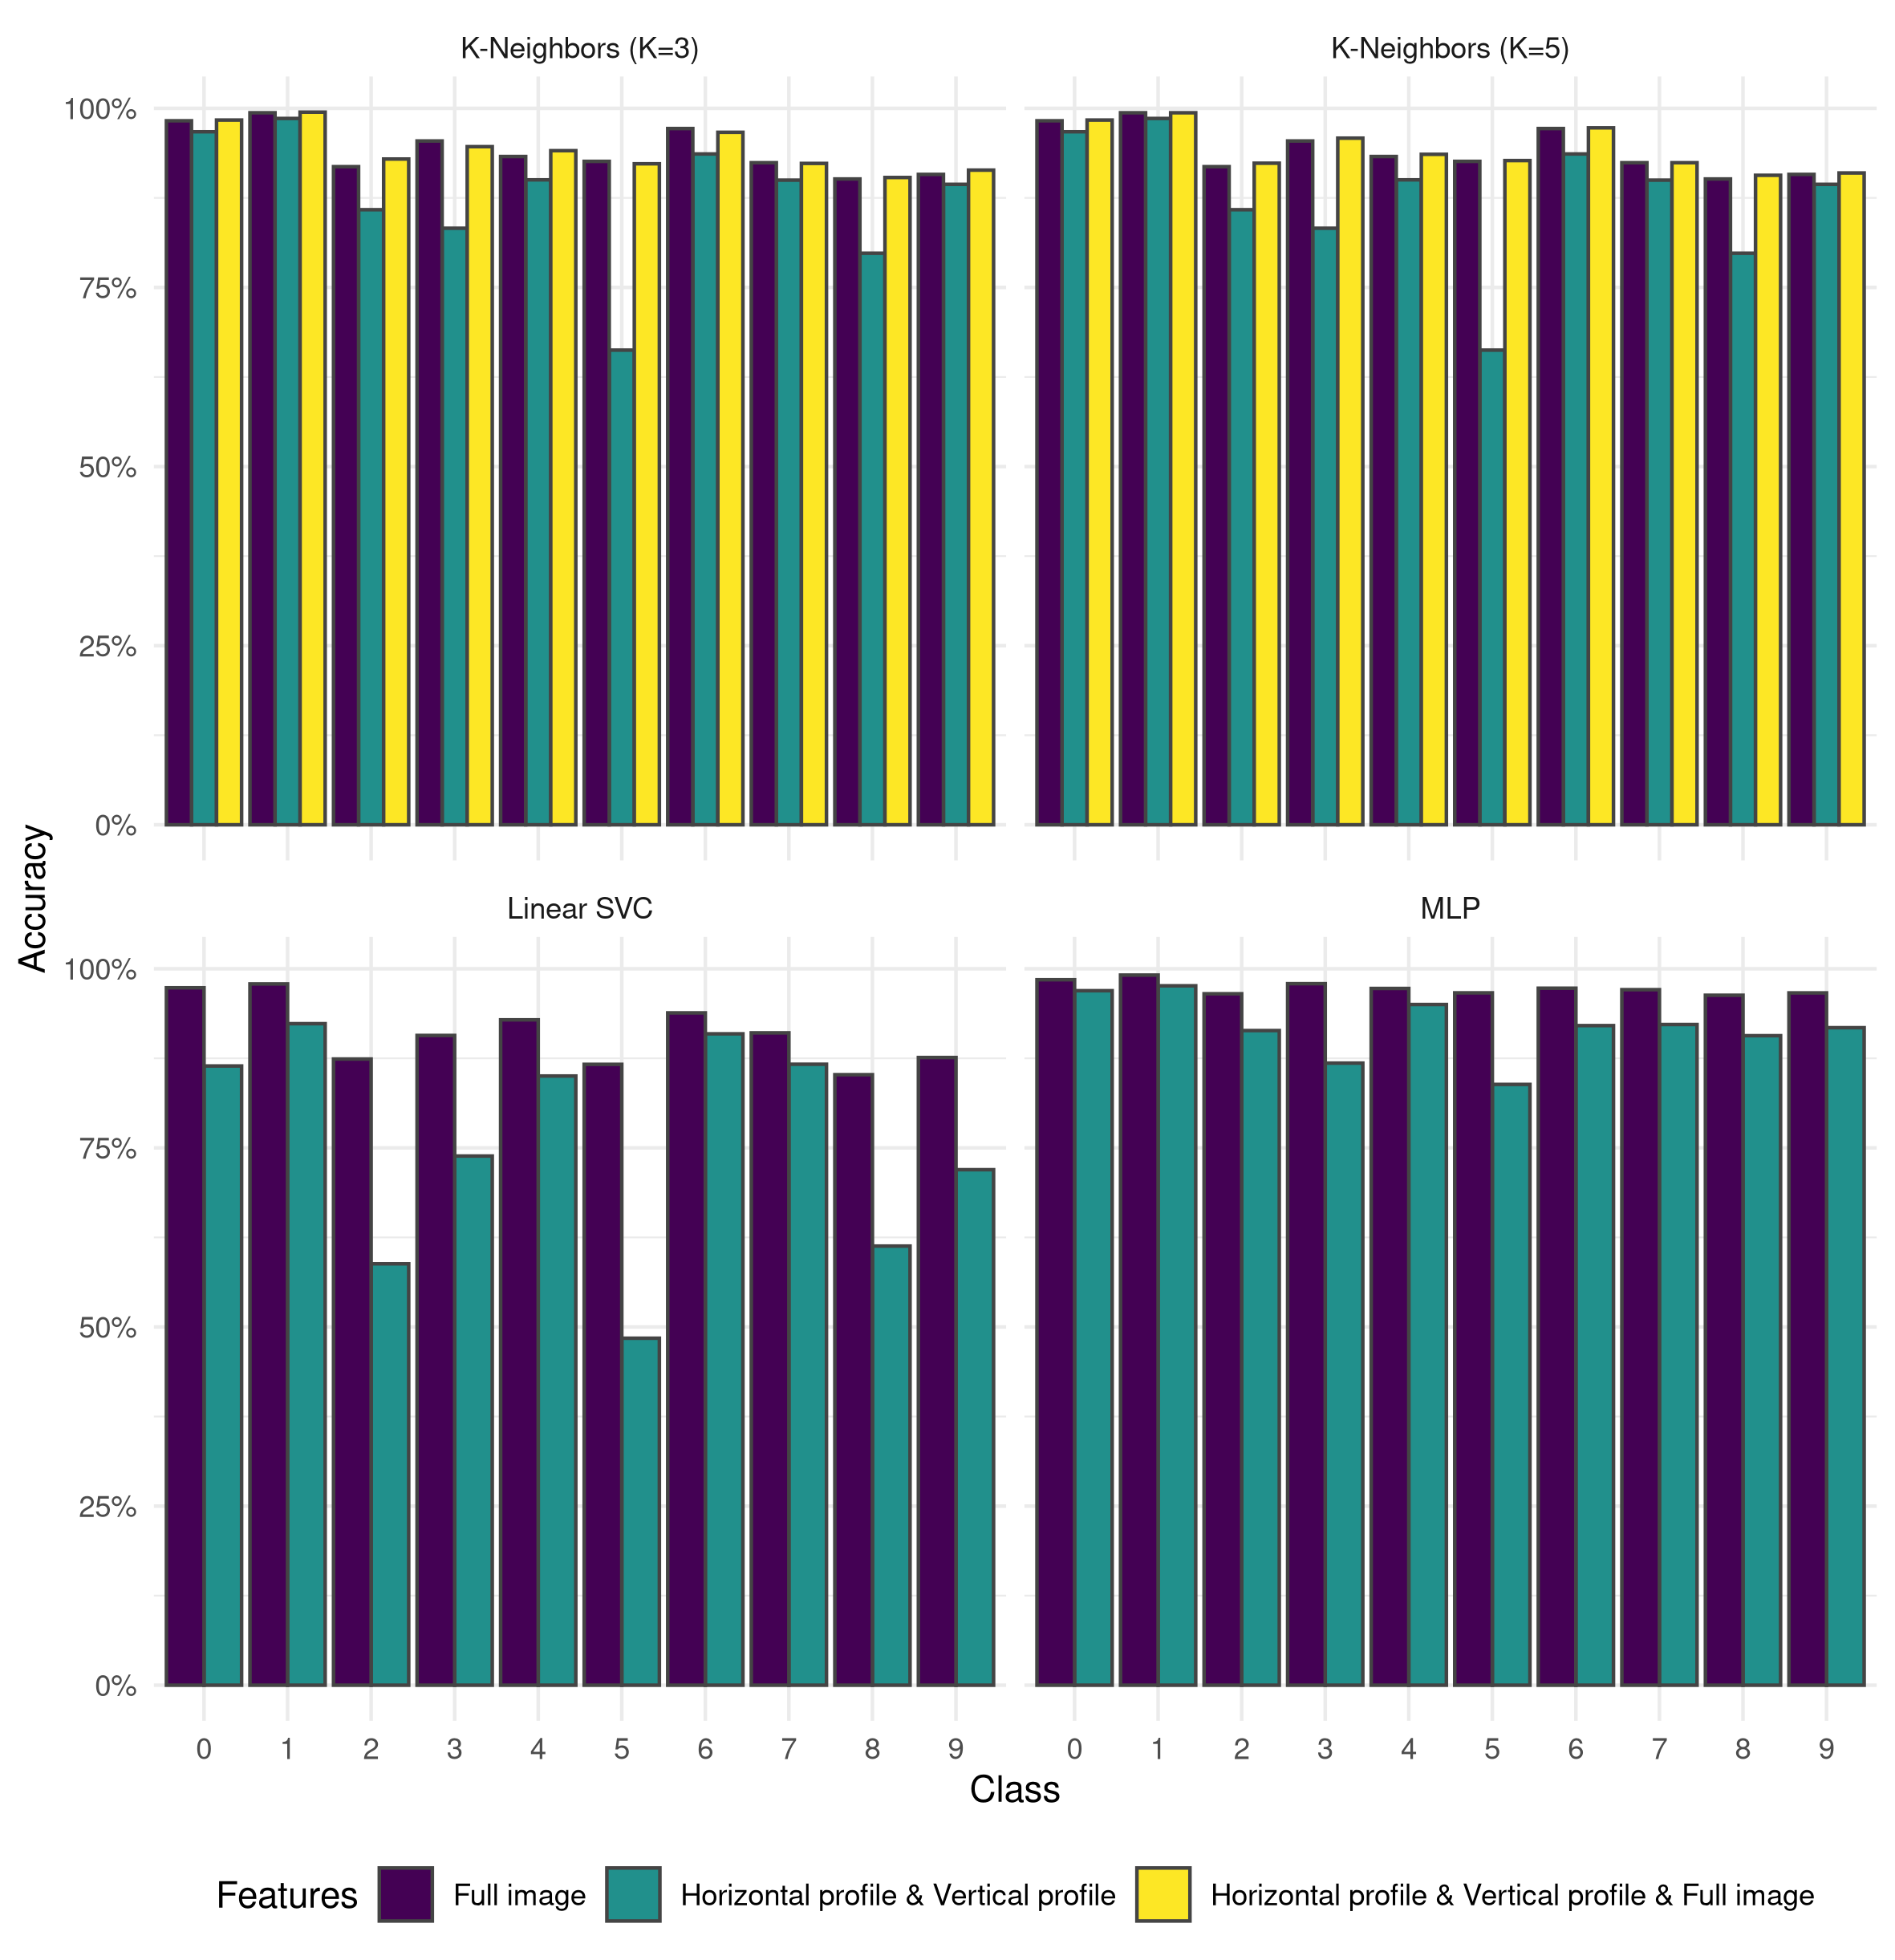
\includegraphics[width=\textwidth]{../resources/scikit_overview.png}
		\caption{Prediction accuracy}
		\label{fig:scikit_accuracy}
\end{figure}

\begin{table}
		\begin{tabular}{lllll}
				\toprule
				Classifier & Features & Average & Worst & Best \\
				\midrule
				K-Neighbours ($K = 3$) & Full image & \SI{94}{\percent} & \SI{90}{\percent} & \SI{99}{\percent} \\
				K-Neighbours ($K = 3$) & Horizontal \& vertical profile & \SI{87}{\percent} & \SI{66}{\percent} & \SI{99}{\percent} \\
				K-Neighbours ($K = 3$) & Horizontal \& vertical profile \& full image & \SI{94}{\percent} & \SI{90}{\percent} & \SI{99}{\percent} \\
				K-Neighbours ($K = 5$) & Full image & \SI{94}{\percent} & \SI{90}{\percent} & \SI{99}{\percent} \\
				K-Neighbours ($K = 5$) & Horizontal \& vertical profile & \SI{87}{\percent} & \SI{66}{\percent} & \SI{99}{\percent} \\
				K-Neighbours ($K = 5$) & Horizontal \& vertical profile \& full image & \SI{94}{\percent} & \SI{90}{\percent} & \SI{99}{\percent} \\
				Linear SVC & Full image & \SI{91}{\percent} & \SI{85}{\percent} & \SI{98}{\percent} \\
				Linear SVC & Horizontal \& vertical profile & \SI{76}{\percent} & \SI{48}{\percent} & \SI{92}{\percent} \\
				MLP & Full image & \SI{97}{\percent} & \SI{96}{\percent} & \SI{99}{\percent} \\
				MLP & Horizontal \& vertical profile & \SI{92}{\percent} & \SI{84}{\percent} & \SI{98}{\percent} \\
				MLP & Horizontal \& vertical profile \& Full image & \SI{96}{\percent} & \SI{94}{\percent} & \SI{98}{\percent} \\
				\bottomrule
		\end{tabular}
		\label{tbl:scikit_accuracy}
		\caption{Feature statistics}
\end{table}

\section{Conclusion}

This has shown that, even with very basic features and a naive classifier,
accuracy suitable for at least supporting a human operator can be achieved.
Using actual industry-standard classifiers then provides prediction accuracy
approaching levels which can be acceptable for unsupervised operation.

It was shown to be beneficial to provide the classifiers access to the full
image data rather than to aggregations if training time permits.

Classifiers such as MLP have been shown to be performant enough that training
on a large set can be done in a reasonable time on modern hardware, while
simultaneously having good prediction accuracy.

Prediction time has been low enough for all classifiers that it is of no
concern.

It is likely that prediction accuracy can be further improved by tuning model
parameters, and suitably preprocessing data.

\end{document}
